\chapter{Exoplanets and Brown Dwarfs}
\label{ch:exo}
Extrasolar planet research has similarities with EB studies in the sense that similar data, 
light, and radial velocity curves are used. A star-planet system, or low-luminosity object like brown dwarfs, 
with transits and radial velocities for the star only, is in many respects analogous to a single-lined spectroscopic and detached EB.

There has been a long history of claims of detection of extrasolar planets, but only in recent 
decades such claims became verifiable and, indeed, have been verified. 
\cite{Campbell1988} tentatively reported the detection of a planet in orbit around the star $\gamma$
Cephei, but this was not confirmed conclusively until 15 years later \citep{hatzes2003}. 
The first confirmed detection of extrasolar planets was by \cite{wolszczan1992} 
around the pulsar PSR 1257+12. In 1995, \cite{Mayor1995} made the
first unambiguous discovery of a planet around a main sequence star: 51 Pegasi. The
planet turned out to be more massive than Jupiter, and in close proximity to the star, a
characteristic that earned it and subsequently discovered similarly placed objects the
nickname \textquote{hot Jupiters}. Thus far, this and most of the extrasolar planets discovered
to date have been identified through radial velocity variations of the orbited stars \citep{kallrath2009eclipsing}.

As the number of detected transiting planets increases (on March 1, 2017, the Extrasolar
Planet Encyclopedia listed 3586 planets in 2691 planetary systems \citep{exoplanetwebsite}), EB analyzing methods become
more and more important to extrasolar planet researchers. In favorable cases they
can give the mass ratio, inclination, as well as period, rate of period change, semi-major axis, 
stellar, and planetary radius \citep{kallrath2009eclipsing}.

%Several of the search methods for extrasolar planets and brown dwarf are similar to those employed to
%search for eclipsing and other periodic variable stars, but need to be more exacting
%because of the low amplitudes involved. At present there are five direct and a few
%indirect methods available in the search for extrasolar planets:
%\begin{itemize}
%\setlength\itemsep{0em}
%\item astrometric variations;
%\item (direct) imaging/spectroscopy of planets and brown dwarfs;
%\item gravitational lensing;
%\item radial velocity variations;
%\item transits;
%\item indirect effects of planets and brown dwarfs on (O-C) diagrams of EBs, and on stellar disks such as warps, gaps, and clumps.
%\end{itemize}
\section{Definition of Exoplanet and Brown Dwarf}
Derived from the solar system analogy, exoplanets designate small bodies orbiting around
stars and formed by condensation in a circumstellar dust disk. 
A first question is, of course, how small has the body to be for being a planet. 
The problem here is that there are small bodies orbiting stars which are probably not formed
like planets, namely brown dwarfs forming, like stars, by collapse of a (possibly dusty) gas cloud.

%One could be tempted to think that the more massive the object is, the larger it is in size and that 
%there is some limit in mass and/or radius beyond which objects are not planets but
%very low mass stars below the 80 Jupiter mass limit to trigger nuclear fusion (namely “brown dwarfs”). 
%The mass on radius dependence (see Fig.\ref{fig_exbd}) shows that there is no clear mass-radius
%relation.

We are dealing with two problems: terminology (what is a planet? what is a brown dwarf?) and classification
(how to decide if a given object is a planet or a brown dwarf according to a given definition?). 
Assuming that the definition of a planet and a brown dwarf is adopted according to their formation mechanism, the separation 
of the two populations is not an easy task \citep{COROT_book}.
%Let us discuss these two aspects.
Let us discuss the formation scenarios of both types of objects and made the conclusions.

%\begin{figure}[!ht]
%\vspace{0cm}
%\centerline{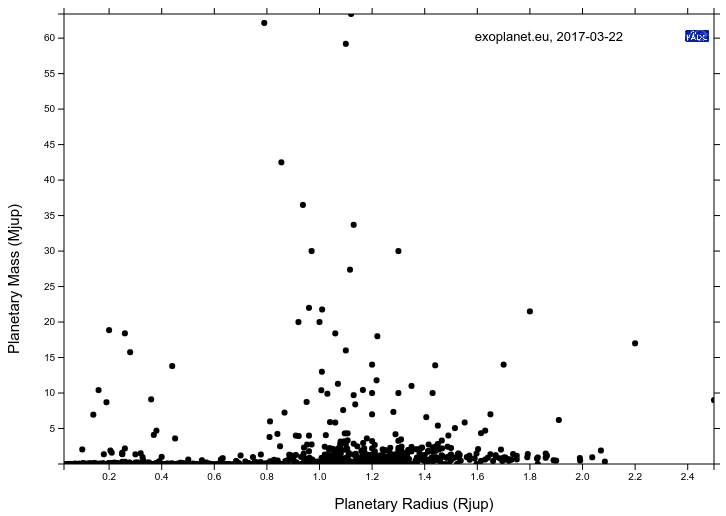
\includegraphics[width=0.80\textwidth]{exoplanets_MR_2.png}}
%\caption{Mass-radius relation for objects confirmed in planetary status\\ (on 22 Mar 2017), from \url{www.exoplanet.eu}}
%\label{fig_exbd}
%\end{figure}

%Conceptual discrimination between planets and brown dwarfs is based on a criterion involving an inobservable
%concept, namely its formation scenario, because we do not have the formation movie at hand. We can only rely
%on actual observables. Standard basic bulk observables are the object mass, radius, temperature. 
%An ideal situation would be that, at least for one of these observables, there
%are two domains $D_{p}$ and $D_{bd}$ of values which
%do not intersect. It is unfortunately not the case since there
%are planets smaller or larger, heavier or lighter, cooler or hotter than objects we believe to be brown dwarfs. 
%The choice made by the Extrasolar Encyclopaedia at exoplanet.eu, based on \cite{Hatzes2015}, is to take
%all objects below 60 Jupiter mass as planet.
%
%The \cite{Hatzes2015} argument is that the mass-radius and the mass-density relations presents no particular feature
%in the giant planet regime (i.e. more massive than Saturn) and that there is a change in the slope of distribution
%at 60 Jupiter mass (see Fig.\ref{fig_ajl2015}). 
%But unfortunately their statistics in the 30-60 Jupiter mass region is poor (the so-called desert) 
%since they rely only on transiting planets and do no consider the mass histogram in
%this region. Earlier data suggested a dip around 40 Jupiter mass \citep{Sahlmann2011, Udry2010} in the mass histogram. 
%More statistics will come in the near future, including radial velocity data from
%the ground and astrometric data from Gaia, to see if a feature around 40 Jupiter mass in the mass-radius diagram
%exists or not.
%
%\begin{figure}[!ht]
%\vspace{0cm}
%\centerline{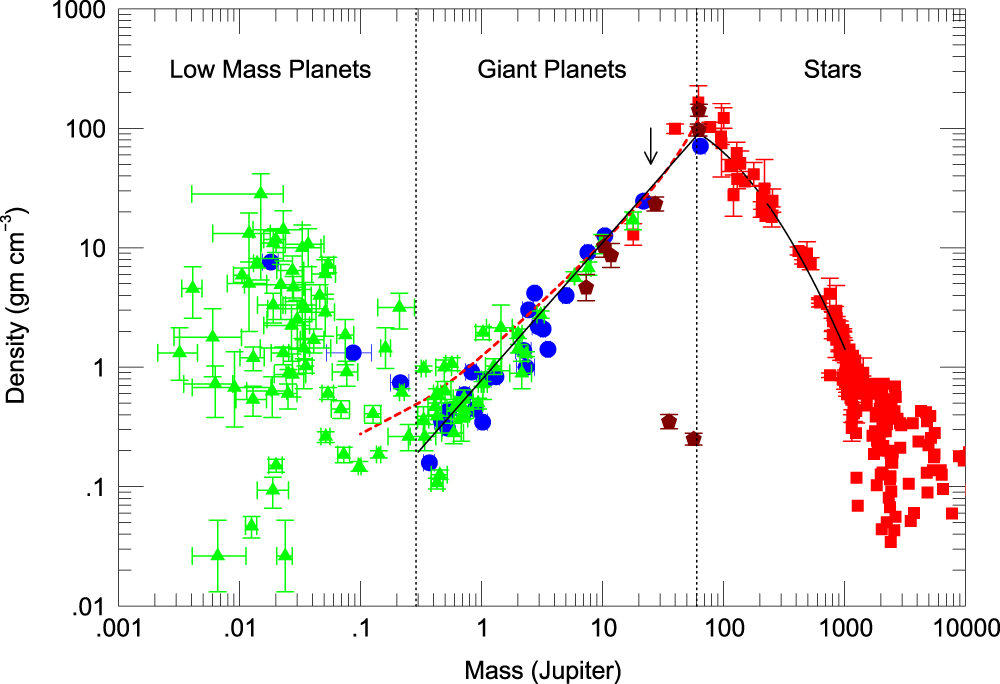
\includegraphics[width=0.80\textwidth]{apj2015.png}}
%\caption{Empirical mass-density relation. \textcopyright \cite{Hatzes2015}}
%\label{fig_ajl2015}
%\end{figure}
%
%A future improvement to separate the planet and brown dwarf populations will come from advanced observables,
%like the spectral type and species composition. They will help to constrain the formation mechanism of the object
%(accretion in a dust disk or collapse of a gas cloud).
%
%At least one conclusion is clear, the former mass limit of exoplanets at 13 Jupiter mass, corresponding to the triggering
%of nuclear burning of Deuterium, is not relevant since an object can be formed by dust accretion and acquire a
%final mass greater than 13 Jupiter.
%There is a second, more factual, problem: the value of observables can be very uncertain. This is especially the
%case for objects detected by imaging where the mass cannot be inferred from radial velocity measurements but only from
%spectra and models.
%The last problem, which we do not consider here because the concerned population is generally supposed to be small,
%is the “interstellar wanderers”, i.e. planets ejected by dynamical interaction from a well-formed planetary system.
%
%Assuming that the definition of a planet and a brown dwarf is adopted according to their formation mechanism, the separation 
%of the two populations is not an easy task \citep{COROT_book}.

\section{Common formation scenario: disk fragmentation}
\label{sect:formation_disk}

Disk fragmentation has been invoked both for the formation of brown dwarfs (BD) and giant planets (GP) and thus its pertinence must be examined as a general mechanism for the formation of sub stellar objects (SSO). 

The disk must be massive enough and fulfill the appropriate cooling conditions to become gravitationally unstable and lead eventually to the formation of GP or BD companions. 
Some simulations \citep{Stamatellos2007, Vorobyov2006} do predict BD formation at large orbital distances under such conditions, 
if the disk is massive and extended enough (typically $M_d\gtrsim 0.3\,\,M_\star$, $R_d\gtrsim 100\,(M_\star/ M_\odot)^{1/3}$ AU \citep{Stamatellos2009}). 
These simulations, however, lack a fundamental physical ingredient, namely the magnetic field. Indeed, it has been shown by several studies that magnetic fields prevent significant 
mass growth and stabilize the disk, severely hampering fragmentation \citep[e.g.][]{Hennebelle2008b,Price2009,Commercon2010,Machida2010}. 
Magnetic fields drive outflows and produce magnetic breaking, carrying out most of the angular momentum. 
These simulations, however, were conducted with ideal MHD. Subsequent calculations have shown that non-ideal MHD effects \citep[e.g.][]{Dapp2012,Machida2011b}, misalignment of the field with the rotation axis \citep{Hennebelle2009b,Joos2012,Li2013} 
and the turbulent nature of the velocity field \citep{Joos2013,Seifried2012,Seifried2013} all decrease the efficiency of magnetic braking. 
However, although large discs can form in these cases, they still remain smaller and less massive than the ones produced in pure 
hydrodynamical simulations. 
Three-dimensional calculations including radiation hydrodynamics, turbulence and complete MHD equations suggest that, for typical observed values of cloud magnetizations and rotation rates, large Keplerian disks do form during the initial core collapse phase
but do not seem to be massive enough to lead to fragmentation. 
This importance of magnetic field has received strong support from the confrontation of observations carried out at the PdBI with synthetic images derived from simulations of both pure hydro and MDH simulations \citep{Maury2010}. It was shown that the disk synthetic images derived from the MHD simulations were similar to the observed ones, with rather compact disks of typical FWHM $\sim 0.2^{''}$-0.6$^{''}$, while the hydrodynamical simulations were producing both too much extended disks and too fragmented (multiple) structures compared with observations. Moreover, observations of isolated disks at the early class 0 stage have revealed compact ($R\sim 20$ AU) disks \citep{Rodriguez2005}, 
while so far extended {\it massive} disks prone to fragmentation appear to be rare. Although better statistics is certainly needed to reach more robust conclusions.
Therefore, although disk fragmentation probably occurs in some disks at the early stages of star formation, 
the fragmentation process is largely overestimated in purely hydrodynamical simulations. Furthermore it is not clear
that fragments, if they form in the disk, will be able to cool quickly enough to form bound objects and to survive turbulent motions or rotational shear nor that they will not migrate quickly inward and end up been accreted by the star, leading to
episodic accretion events.

Other observational constraints seem to contradict gravitational instability (GI) in a disk as the {\it main route} for
BD or GP formation. If indeed this mechanism was dominant, most Class 0 objects should have massive disks, a conclusion which does not seem, 
so far, to be supported by observations. An argument sometimes raised by some proponents of this scenario \citep[e.g.][]{Stamatellos2009} is that the lifetime of the massive and extended disks produced in the simulations is too short ($\sim$ a few 10$^3$ yr) for the disks to be observed. This argument, however, does not hold since Class 0 objects last over a significantly longer period, about $\sim 10^5$ yr.
%, leaving statistically sufficient opportunities to see such massive disks.
Second of all, these simulations do not include an accreting envelope and thus end up too early compared with realistic situations, yielding an inaccurate diagnostic. 
As mentioned above, more accurate calculations including accreting envelope, magnetic field, turbulence and feedback (e.g. \citet{Seifried2013}; Masson et al., in prep.) show the emergence of large centrifugal disks but, for typical observed magnetic flux conditions, the disks do not appear to be massive enough to lead to fragmentation, at least for low mass protostars, the bulk of the
distribution. It is fair to say, however, that at the time these lines are written this important issue is far from being settled and further exploration of this topic is needed. As mentioned above, however,
it is mandatory to include all the proper physics in these studies to reach plausible conclusions. 

Most importantly, the observational constraints arising from the existence of wide BD or GP companions strongly argue against GI as an efficient formation mechanism. 
%An interesting exemple is the triple system LHS6343 \citep{Johnson2011}, with the presence of a BD companion with mass $M_C=0.063\, M_\odot$ to a low-mass star with $M_A=0.37\, M_\odot$. 
%Assuming disk-to-star standard mass fractions around $\sim 10\%$, the disk around $M_A$ should thus have a mass $M_d\approx 0.04\, M_\odot$. Although admittedly crude, this estimate shows that there is not enough mass in the disk to have formed the BD companion, even if assuming 100\% disk-to-BD mass conversion efficiency. 
Finally, the statistics arising from direct imaging revealing, at least so far, the scarcity of wide and massive SSO's in the BD or GP mass range around FGKM-type stars strongly argues against GI as the {\it main} formation mechanism for BD's or GP's. 
One might invoke the possibility that objects form by GI at large orbits and then migrate inwards closer to the star. 
This argument, however, does not hold. First, it must be stressed that
the possibility of migration is already included in the general analysis mentioned above. Secondly, if there was a "planetary" population forming by GI and migrating inwards, there should also be a "brown dwarf" population undergoing the same process. But this can be firmly observationally excluded. Finally, if we interpret the existing close-in planet population as objects that
formed by GI and migrated inwards, this would not explain planet bottom-heavy mass distribution and planet-metallicity correlation.
Gravitational instability, however, might occur in some particular situations, like for instance in very massive disks around {\it binary systems} \citep{Delorme2013}, even though other formation mechanisms are also possible in such situations.
The combination of ALMA and future direct imaging projects will definitely help nailing down this issue.

\section{Formation Scenarios For Brown Dwarfs}

\subsection{Photoionization}
The fact that the brown dwarfs (BD) mass function is about the same regardless of the presence or not of O stars shows that halting
of accretion by photoionizing radiation \citep{Whitworth2004} is clearly not a major mechanism for BD 
formation. Furthermore BD’s have been observed in isolated environments, excluding a necessary
connection between the presence of photoionizing radiation and BD formation.

\subsection {Accretion-ejection}
In the accretion-ejection scenario \citep{Reipurth2001}, BD’s are the result of accreting $\sim 1~M_{Jup}$ stellar
embryos, formed by the efficient dynamical fragmentation of a molecular clump, which get ejected from the surrounding 
gas reservoir and in the end remains in the sub-stellar domain. The characteristic conditions of this scenario are
(1) that dynamical interactions are responsible for the formation of both high-mass (by merging) and low-mass (by
ejection) objects, implying that star formation occurs basically, if not only, in dense cluster environments, 
(2) that the initial mass function (IMF) is determined essentially at the latest stages of the collapse, namely the ultimate gas-to-star conversion, with no correlation whatsever with the initial core mass function. 
In fact, pre-stellar cores do not really exist in this scenario.

The most achieved simulations exploring this scenario are made by \cite{Bate2012} which, although still
lacking magnetic field, include a treatment of gas heating and cooling. One of the most striking results of these 
simulations is that the resulting IMF reproduces quite well the \cite{Chabrier2005} IMF. These simulations, 
however, remain of questionable relevance for most Milky Way (MW) molecular cloud conditions. Indeed, it has been 
established observationally that star forming molecular clouds in the MW follow the so-called Larson’s relations \citep{Larson1981}, 
although with significant scatter, in terms of cloud size vs mean density and velocity dispersion 
(e.g. \citep{Hennebelle2012}): 
%$ \bar{n} \simeq 3 \times 10^3 \left( \frac{L}{1pc}\right)^{-\eta_d} ~cm^{-3} $,
%$\sigma_{rms} \simeq 0.8 \left( \frac{L}{1pc}\right)^{\eta} ~km~s^{-1}$ 
\begin{equation}
\bar{n} \simeq 3 \times 10^3 \left( \frac{L}{1~pc}\right)^{-\eta_d} ~cm^{-3}
\end{equation}

\begin{equation}
\sigma_{rms} \simeq 0.8 \left( \frac{L}{1~pc}\right)^{\eta} ~km~s^{-1}
\end{equation}
with $\eta_d \sim 0.7-1.0$ and $\eta \sim 0.4$.
Bate’s (2012) initial conditions, however, correspond to a 500 $M_{\odot}$ cloud at 10 K with size $L = 0.4~pc$, thus mean density 
$\bar{n} \simeq 3.2 \times 10^4 ~cm^{−3}$ and surface density $\Sigma \simeq 10^3 ~M_{\odot} ~pc^{−2}$ 
(while typcal values for MW molecular clouds are around $\sim 60-100 M_{\odot}~ pc^{−2}$ \citep{Heyer2009}). % and Mach number ${\cal M}=14$. 
These values correspond to rather extreme cloud
conditions, about 4 to 5 times denser and more turbulent than the aforementioned typical observed ones. Such conditions 
will support fragmentation and dynamical interactions and it is thus not surprising that they produce a
significant number of ejected BD embryos. Interestingly enough, these simulations can be directly confronted to 
observations. 
%Indeed, the simulated cloud mass and size are very similar to the ones of the young cluster NGC1333. 
%The simulations, however, produce a significantly larger number of stars+BD’s than the observed
%ones, with a total stellar mass $\sim 191\,M_\odot$ against $\sim 50\,M_\odot$ in NGC1333 \citep{Scholz2012a}; interestingly, this echos
%the aforementioned factors $\sim$ 4 in density and velocity.
Other inputs in the simulations, for instance the assumption of a uniform initial density profile, the lack of magnetic
field, and the underestimated radiative feedback all support fragmentation and thus probably overestimate the number
of proto-stellar or proto-BD embryos formed in a collapsing core, again supporting dynamical interactions/ejections. 
Observations in fact tend to suggest that fragmentation within pre-stellar cores is rather limited, most of the mass of the
core ending up in one or just a few smaller cores \citep{Bontemps2010, Tachihara2002}. This again
casts doubts on the relevance of such initial conditions to explore star/BD formation under typical Milky Way molecular 
cloud conditions. At least, if indeed BD formation by dynamical ejections might occur under some circumstances, 
existing simulations severely overestimate the efficiency of this process. In fact, one is entitled to suspect
that the similarity between the IMF produced by the simulations and the one representative of the Galactic field reflects
in reality the result of the initial gravoturbulent collapse of the cloud rather than the results of dynamical interactions.
In which case, the IMF in the simulations should already be largely determined at the begining of the simulation. If
this is the case, these simulations in fact bring support to star/BD formation by gravoturbulent collapse. At any rate,
until simulations with more realistic initial conditions are conducted, the ones performed by \cite{Bate2012} cannot be
considered as a reliable demonstration of dominant BD formation by accretion-ejection.

%The accretion-ejection scenario faces other important issues. Without being exhaustive, one can add a few more. (1)
%How can BD’s form, according to this scenario, in low-density environments? The Taurus cloud for instance, even
%though having a stellar density about 3 orders of magnitude smaller than other common clusters, has a comparable 
%abundance of BDs \citep{Luhman2012}. As noted by \cite{2011}, the low stellar density ($\lesssim 5~ stars /pc^2$ ) and
%low velocity dispersion of Taurus members ($\sigma \sim 0.2~ km~ s^{−1}$ ), indicate that there is no small N-body clusters from
%which stars or BDs could have been ejected, as advocated in the accretion-ejection scenario. The fact that BD’s form
%as efficiently in such low-density environments strongly argues against dynamical interactions. (2) Various observations 
%show average dispersion velocities of pre-stellar cores of about  $\langle \sigma \rangle \sim 0.4~ km~ s^{−1}$ \citep{Andr2009, Walsh2007, Muench2007, Gutermuth2009, Bressert2010}. This indicates a typical collision timescale 
%between pre-stellar cores significantly larger than their dynamical timescale, suggesting little dynamical evolution during
%pre-stellar core formation. (3) How can this scenario explain the observed similarity between the CMF and the IMF, if
%indeed such a similarity is confirmed?

All these observational constraints (notably the observed small velocity dispersion between protostar/BD’s) severely
argue against the accretion-ejection scenario for BD or star formation as a dominant mechanism, except possibly for
the most massive stars, which represent only a very small fraction of the stellar population.


\subsection{Gravoturbulent Fragmentation}
\label{sec:gravo}

In this scenario, large-scale turbulence injected at the cloud scale by various sources 
cascades to smaller scales by shocks and generates a field of density fluctuations down to the dissipative scale \citep[e.g.][]{MacLow2004}. Overdense regions inside which gravity overcomes all other sources of support collapse and form self-gravitating cores which isolate themselves from the surrounding medium. In this scenario, the mass function of pre-stellar cores (CMF) or IMF is set up by the spectrum of turbulence, at the very early stages of the star formation process. 
The first theory combining turbulence and gravity was proposed by \cite{Padoan2002} but has been shown to suffer from various warnings 
\citep[e.g.][]{McKee2007, Hennebelle2011a}. 
%Moreover, it requires the presence of a magnetic field to yield the proper IMF, in contrast to simulations. 
A different theory was derived more recently by \cite{Hennebelle2008a,Hennebelle2009a, Hennebelle2013} and \cite{Hopkins2012}. These latter theories nicely reproduce the IMF down to the least massive BDs, for appropriate conditions. The important feature
of these theories is that it is inappropriate to use the average thermal Jeans mass as an estimate of the characteristic mass for fragmentation. This would of course preclude significant BD formation. Indeed, in both Hennebelle-Chabrier and Hopkins theories, the spectrum of collapsing prestellar cores strongly depends on the Mach number, shifting the low-mass tail of the IMF to much smaller scales than naively expected from a purely gravitational Jeans argument. The theories indeed yield a reasonably accurate number of pre-BD cores for adequate molecular cloud like conditions and Mach values (${\cal M}\sim 3-8$). Densities required for the 
collapse of BD-mass cores, $\sim 10^7$-$10^8$ g cm$^{-3}$, are indeed produced by turbulence induced shock compression 
% (remembering that shock conditions imply density enhancements $\propto{\cal M}^2$). 
%Note that a similar scenario, taking into account the filamentary nature of the star forming dense regions, was developed by \cite{Inutsuka2001} (see chapter by {\it Andr\'e et al.}). 

Support for the gravoturbulent scenario arises from several observational facts. (1) It explains, within the framework of the same theory, the observed mass spectra of both {\it unbound} CO-clumps and {\it bound} prerestellar cores \citep{Hennebelle2008b}; (2) it implies that the IMF is already imprinted in the cloud conditions (mean density, temperature and Mach number), naturally explaining the resemblance of the CMF with the IMF; (3) it relies on one single "universal" parameter, namely the velocity power spectrum index of turbulence, which explains as well the Larson's relations for molecular clouds.

A major problem against the gravoturbulent scenario to explain the {\it final} IMF would arise if the cores were fragmentating significantly into smaller pieces during their collapse. Observations tend to show that
such fragmentation is rather limited. Numerical simulations of collapsing dense cores indeed show that radiative feedback and magnetic fields drastically reduce the fragmentation process \citep[e.g.][] {Krumholz2007, Offner2009, Commercon2010, Commercon2011, Hennebelle2011b,Seifried2013}. 
The analysis of simulations aimed at exploring the CMF-to-IMF conversion \citep{Smith2009} also show a clear correlation between the initial core masses and the final sink masses up to a few local freefall times \citep{Chabrier2010}, suggesting that, at least for the
bulk of the stellar mass spectrum, the initial prestellar cores do not fragment into many objects, as indeed suggested by the CMF/IMF similarity. But the most conclusive support for BD formation by gravoturbulent fragmentation comes from the emerging observations of isolated proto-BD's and of the pre-BD core Oph B-11\citep{Chabrier2014}.

\subsection{Formation of Binaries}
\label{bin_fn}

Newly formed stars must disperse a tremendous amount of angular momentum in condensing through more than 6 orders of magnitude in radius \citep{Bodenheimer1995}. Besides magnetic braking, binary formation offers a  convenient way
to redistribute at least part of this excess angular momentum. 

Several binaries have been observed at large {\it projected} separations ($>500$ AU) with masses down to $\sim 5\,M_{Jup}$. \cite{Looney2000} showed that multiple systems in the Class 0 and I phases are prevalent on large spatial scales ($\gtrsim$ 1000 AU) 
while binary systems at smaller scales ($\lesssim$ 500 AU) seem to be quite sparse \citep{Maury2010}.
Whether this lack of small scale binaries at the Class 0/I stages is real or stems from a lack of observations with sufficient resolution or sensitivity, however, is still unclear so far.
In any case, prestellar and protoplanetary disks do not extend out to thousand AU's so
formation of such wide BD binaries by disk gravitational instability (GI) seems to be clearly excluded. In contrast, such distances can be compared with the characteristic sizes of starless prestellar core envelopes, $\sim 10^4$ AU \citep{Menshchikov2010}. The existence of these wide systems thus suggests
that prestellar core fragmentation into binaries might occur at the very early stages of the collapse. Indeed, there are some observational evidences for binary fragmentation at this stage \citep{Looney2000,Duchene2003}. Moreover, the similarity, at least in a statistical sense, between some of the star and BD multiplicity properties suggests that most BD companions form similarly as stellar companions. This hypothesis has received theoretical 
and numerical support
form the recent work of \cite{Jumper2013}. These authors show that BD properties, including the BD desert, wide BD binaries and the tendency for low-mass (in particular BD) binaries to be more tightly bound than stellar binaries, arguments often used as an evidence for distinct formation mechanisms for BD's, can de adequately reproduced by angular momentum scaling during the collapse of turbulent clouds. 
Indeed, the early stages of cloud collapse/fragmentation and core formation are characterized by the formation of puffy disc-like structures which keep accreting material 
from the surrounding core envelope. These structures, however, are not relaxed and differ from structures purely supported by rotation, characteristic of relaxed, equilibrium discs.
Such "pseudo-discs" may fragment (as the result of global non-linear gravitational instability) during the (first or second) collapse of the prestellar core and end up forming (wide or tight) binaries, 
possibly of BD masses \citep{Bonnell1994, Machida2008}. 
The occurence of such fragmentation at the cloud collapse stage has been found in radiation-hydrodynamics simulations \citep{Commercon2010, Peters2011, Bate2012}. 
They remain to be explored in the context of resistive MHD before more definitive conclusions can be reached concerning this important issue. 
Such fragmentation into binaries occurs at the {\it very early stages of the core collapse}, during the main accretion phase. 
%They thus differ from the usual disk GI which involves a local, linear (Toomre) in a centrifugally supported disc. 
Whether it occurs dominantly by redistribution of angular momentum during the collapse itself or by global instability in the mass loaded growing pseudo-disk remains so far
 an open question and a clear-cut 
distinction between the two processes is rather blurry at this stage. 
It must be kept in mind, however, that the conditions for the formation {\it and} survival of bound fragments in a disk are subject to very restrictive constraints.


\section{Formation Scenarios For Giant Planets: Core \mbox{Accretion}}
\subsection{Core Accretion Mechanism}
In the core accretion scenario gas-giant planets form in two steps. First, a solid core is accumulated by accretion of
planetesimals. The growing core attracts a hydrostatic envelope of protoplanetary disk gas, extending from the 
surface out to the Bondi radius where the sound speed equals the escape speed of the core. Since accreting planetesimals
not only increase the core mass but also release gravitational energy, the energy released at the core surface must
be transported through the envelope, making the latter non-isothermal. The mass of the envelope increases with the
core mass faster than linearly, so that at some point the envelope starts to dominate the gravitational potential. 
Hydrostatic solutions cease to exist beyond a critical core mass which depends mainly on the accretion rate of solids and on
the gas opacity. As a result, core starts accreting mass on its own thermal timescale, turning itself into a giant planet.
\cite{Perri1974} assumed the hydrostatic envelope to be fully convective and found critical core masses
in excess of 100 Earth masses; they used this result to support the alternative gravitational instability scenario for
giant planet formation. \cite{Mizuno1980} allowed both for convective and radiative regions in the envelope and constructed 
the equilibrium model using gas opacities depending on the density and temperature, with a stepwise constant
dust opacity below the dust sublimation temperature. The radiative solution drastically reduces the critical core mass
to approximately 10 $M_\oplus$ , in agreement with constraints from the gravitational potentials of Jupiter and Saturn 
\citep{Guillot2005}, for an assumed mass accretion rate of $10^{−6} M_\oplus$ per year. Planetary envelopes can still be fully convective
at very high planetesimal accretion rates \citep{Wuchterl1993, Ikoma2001, Rafikov2006}, typical for cores at $\sim$AU
from the star, but this is unlikely to be an issue at large separations (Rafikov, 2006).
A generic property of the hydrostatic envelope is that its mass is inversely proportional to the luminosity (and hence
to the mass accretion rate) and to the opacity \citep{Stevenson1982}. The resulting critical core mass roughly scales as
$M_c \propto M^{1/4}$ \citep{Ikoma2000}. Hence the growth rate of the core partially determines the critical core mass. 
Beyond the critical core mass the envelope will emit more energy than provided by the gravitational potential release
of the accreted solids and undergo run-away contraction on the Kelvin-Helmholtz time-scale \citep{Bodenheimer1986}. 
Interestingly, the concept of a critical core mass seems to be supported observationally by the mass-radius
relationship of the recently detected Kepler low-mass transit planets \citep{Lissauer2011a, Lissauer2011b, Carter2012, Ofir2013}, 
bearing in mind the uncertainties in Kepler objects mass determinations. Indeed, while planets above
about $\sim 6 M_\oplus$ seem to have a radius requiring a substantial ($\gtrsim10$\% by mass) gaseous H/He envelope, so far planets 
below this mass have a radius consistent with a much lower, or even negligible gas mass fraction. 
%Even the rather extended
%gaseous envelope of the lowest transiting planet discovered so far, KOI-314c ($1.0^{+0.4}_{−0.3} M_{\oplus}$) (Kipping et al., 2014), 
%with a radius $R_{env} \sim 7^{+12}_{-13}$ \% of the planet’s radius, represents a negligible fraction ($\lesssim$ 3\%) of its mass.

\subsection{Time-scale for accumulation of the core}
In the classical core accretion scenario, the core grows by accreting planetesimals. The Hill radius
\begin{equation}
R_H = [G M_p /(3 \Omega^2 )]^{1/3} = 1/p R_p
\end{equation}
denotes the maximal distance over which the core can deflect planetesimals which pass by with the (linearized) Keplerian shear flow. 
Here $p = (9M_\star /4\pi \rho a^3 )^{1/3} \ll 1$ is a parameter that depends on semi-major axis $a$ and 
material density $\rho$ for a given stellar mass $M_\star$ (Goldreich et al.,2004). An additional random 
component to the particle motion will reduce the scattering cross section of the core to below $\sim R^2_H$.

The gravitational radius of the core denotes the maximum impact parameter at which a planetesimal approaching 
with velocity $v$ gets accreted by a core with radius $R$ at closest approach. This distance is given by
$R_G = R \sqrt{1+\frac{v^2_e}{v^2}}$
where $R$ is the radius of the core, $v_e$ the escape speed at the surface and $v$ the relative approach speed. In dynamically
cold discs planetesimals enter the Hill sphere of the core with the Hill speed $v_H = ΩR_H$ . In that case the gravitational 
radius can be simplified as $R_G \approx \sqrt{p R_H}$. 
A small fraction of the planetesimals which enter the Hill sphere of the core actually collide with it. 
The mass accretion rate is ultimately set by the gravitational radius and the
scale height of the planetesimals. The random motion of planetesimals enter both these quantities and should ideally
be calculated self-consistently using an N-body approach (\cite[e.g.][]{Levison2010}.

Assuming that the random particle motion is similar to $\Omega R_H$ — the Keplerian velocity shear across the Hill 
radius, one can find that the core grows at the rate \citep{Dones1993}
\begin{equation}
dR/dt\sim p^{-1}\Sigma_s\Omega/\rho\approx 50\,\,{\rm m\, yr}^{-1}(r/{\rm AU})^{-2},
\label{eq:drdt}
\end{equation}

Fragment accretion assuming surface density of solids typical for the minimum mass solar nebula (MMSN) ($\sim 30 g cm^{−2}$ at 1 AU). 
This corresponds to the mass growth rate of order $10^{−6} M_\oplus /year$ at 5 AU where Jupiter
presumably formed \citep{Dodson-Robinson2009}. This leads to core formation in $10^7$ years, in marginal agreement
with the observed life times of protoplanetary discs \citep{Haisch2001}, but the time-scale can be brought down by 
assuming a planetesimal column density that is 6-10 times the value in the MMSN (Pollack et al., 1996). Note that
eqn. (\ref{eq:drdt}) assumes uniform planetesimal surface density near the embryo, an assumption which may be violated if
the embryo is capable of clearing a gap in the planetesimal population around its orbit \citep{Tanaka1997, Rafikov2001, Rafikov2003a}, which would slow down its growth \citep{Rafikov2003b}. 

While the agreement between the core mass (or more exactly the total amount of heavy material) of Jupiter and 
the mass accretion rate necessary to form the core is a success
for the core accretion model, the mass accretion rate scales roughly as the semi major axis to the inverse second power
in accordance with equation (\ref{eq:drdt}). Hence core formation beyond 5 AU is impossible in the million-year time-scale of
the gaseous protoplanetary disc. This conflicts both with the high gas contents of Saturn, the small H/He envelope of
Uranus and Neptune and the observations of gas giant exoplanets in wide orbits beyond 10 AU \citep{Marois2008}.

This discussion makes it clear that gas giants can form by core accretion (CA) at large separations only if the core formation timescale
can be reduced dramatically. Ironically, acceleration of the core growth makes it harder to reach the threshold for CA,
because the critical core mass is inversely proportional to the core luminosity, which is predominantly derived from
the heat released in planetesimal accretion. Nevertheless, one can show \citep{Rafikov2011} that higher planetesimal 
accretion rate $\dot{M}$ still reduces the total time until CA sets in, even though the critical core mass is larger and is more 
difficult to achieve.

\subsection{Fragment Accretion}
One pathway to rapid core formation is to accrete planetesimal fragments damped by the gas to a scale height
lower than the gravitational accretion radius \citep{Rafikov2004}. 

Numerical and analytical studies of planetesimal dynamics generically find that soon after a dominant core emerges
it takes over dynamical stirring of the surrounding planetesimals, increasing their random velocities to high values.
Physical collisions between planetesimals then lead to their destruction rather than accretion, giving rise to a 
fragmentation cascade that extends to small sizes. \cite{Rafikov2004} demonstrated that random velocities of particles in a size
range 1 − 10 m are effectively damped by gas drag against excitation by the core gravity. Gas drag also does not allow
such small fragments to be captured in mean motion resonances with the embryo (\cite[e.g.][]{Levison2010}). This
velocity damping is especially effective in the vertical direction, allowing small debris to settle into a geometrically thin
disk with thickness below the maximum impact parameter, still resulting in planetesimal accretion ($\sim p^{1/2} R_H$). From
the accretion point of view the disk of such planetesimal debris is essentially two-dimensional, resulting in the highest
mass accretion rate possible in the absence of any external agents such as described in section \nameref{ss_pebble} below:
\begin{equation}
dR/dt\sim p^{-3/2}\Sigma_s\Omega/\rho\approx 1\,\,{\rm km\, yr}^{-1}(r/{\rm AU})^{-3/2}.
\end{equation}

This formula assumes that most of the surface density of solids $\sum_s$ ends up in small ($\sim$ 10 m) fragments dynamically
cooled by gas drag. Because of the dramatically reduced vertical scale height of the fragment population, this rate
is higher than the previously quoted (\ref{eq:drdt}) for the velocity dispersion $\sim  \Omega R_ H$ and decreases somewhat more slowly
with the distance (as $r^{−3/2}$ ). As a result, a Neptune size core can be formed at 30 AU within several Myrs.
A key ingredient of this scenario is the collisional grinding of planetesimals, which allows them to efficiently 
couple to gas and become dynamically cold, accelerating core growth. Fragmentation plays a role of an agent that transers 
mass from a dynamically hot mass reservoir 
%(population of large planetesimals, accreted at low rate because of relatively weak focussing) 
to dynamically cold debris. Even though at a given moment of time the latter population may
have lower surface density than the former, it is accreted at much higher efficiency and easily dominates core growth.
The importance of fragment accretion for accelerating core growth has been confirmed in recent coagulation simulations 
by \cite{Kenyon2009} (see also \cite{Levison2010}).
In the framework of this scenario \cite{Rafikov2011} sets a constraint on the distance from the star at which gas giants
can still form by CA in a given amount of time (several Myrs). By adopting the maximally efficient accretion of
small debris confined to a two-dimensional disk he showed that giant planet formation can be extended out to 40-50 AU
in the MMSN and possibly even further in a more massive planetesimal disk (out to 200 AU in the marginally gravitationally 
unstable gaseous protoplanetary disk). This estimate makes some rather optimistic assumptions such as
that most of planetesimal mass is in small (1-100 m) objects (e.g. as a result of efficient fragmentation), and that
seed protoplanetary embryos with sizes of at least several hundred km can be somehow produced far from the star
within several Myrs. Thus, it becomes very difficult to explain origin of planets beyond 100 AU by CA. This issue is
examined below.

\subsection{Pebble accretion}
\label{ss_pebble}

The arguably most fundamental particles to accrete are those forming directly by coagulation and condensation as
part of the planetesimal formation process. Several particle growth mechanisms predict that particles will stop growing
efficiently when they reach pebbles of millimeter and centimeter sizes.

While small dust grains grow as fluffy porous aggregates, they are eventually compactified by collisions around
mm sizes and enter a regime of bouncing rather than sticking \citep{Zsom2010}. This bouncing barrier maintains
a component of small pebbles which can feed a growing core. In the alternative mechanism where particles grow
mainly by ice condensation near evaporation fronts, particles sediment out of the gas when reaching pebble sizes.
This reduces their growth rate drastically as they must collectively compete for the water vapour in the thin mid-plane 
layer \citep{Ros2013}. Icy particles may be able to retain their fluffy structure against compactification
and hence avoid the bouncing barrier \citep{Wada2009}, but even under perfect sticking particles grow more slowly
with increasing mass and spend significant time as fluffy snow balls whose dynamics is similar to compact pebbles
\citep{Okuzumi2012}.

The dynamics of pebbles in the vicinity of a growing core is fundamentally different from the dynamics of a planetesimal 
or a planetesimal fragment. Pebbles are influenced by drag forces which act on a time-scale comparable to or
shorter than the orbital period, which is also the characteristic time-scale for the gravitational deflection of particles
passing the planet with the Keplerian shear. The gravity of the core pulls the pebbles out of their Keplerian orbits.
The resulting motion across gas streamlines leads to frictional dissipation of the kinetic energy of the particles and
subsequent accretion by the core. While planetesimals are only accreted from within the gravitational radius, which is
a small fraction of the Hill radius, pebbles are in fact accreted from the entire Hill sphere.

The potential of drag-assisted accretion was explored by \cite{Weidenschilling1985} who showed that particles 
below 1-10 meters in size experience strong enough friction to avoid getting trapped in mean motion resonances
with the growing core. \cite{Kary1993} confirmed these results but warned that only a small fraction (10-40\%) of the
drifting pebbles are accreted by the core due to their radial drift. This concern is based on the assumption that 
pebbles form once and are subsequently lost from the system by radial drift. This loss of solids would be in disagreement 
with observations of dust in discs of Myr age \citep{Brauer2007}. The solution to the drift problem may be that
pebbles are continuously formed and destroyed by coagulation/fragmentation and condensation/sublimation processes
\citep{Birnstiel2010, Ros2013}. Hence, any material that is not immediately accreted by the one or
more growing cores will get recycled into new pebbles that can then be accreted.

\cite{Johansen2010} simulated the accretion of small pebbles onto large planetesimals or protoplanets.
They found that pebbles with friction times less than the inverse orbital frequency are accreted from the entire Hill
sphere, in agreement with the picture of drag-assisted accretion. \cite{Ormel2010} interpreted the rapid 
accretion as a sedimentation of particles towards the core. \cite{Johansen2010} also observed that the pebbles
arrive at the protoplanet surface with positive angular momentum, measured relative to the angular momentum of the
disc, which leads to prograde rotation in agreement with the dominant rotation direction of the largest asteroids.

The dependence of the pebble accretion rate on the size of the core was parameterized in \cite{Lambrechts2012}. 
Below a transition core mass of around 0.01 Earth masses pebbles are blown past the core with the 
sub-Keplerian gas. Pebbles are captured from within the Bondi radius of the sub-Keplerian flow, which is much smaller
than the Hill radius. With increasing core mass the Bondi radius grows larger than the Hill radius, starting the regime
of efficient pebble accretion. Growth rates in this regime are 1,000 times higher than for accretion of large planetesimals
with velocity dispersion of order $\Omega R_H$ (see eqn. (\ref{eq:drdt})), at 5 AU, and 10,000 faster, at 50 AU, depending on the degree
of sedimentation of pebbles. Thus it is possible to make cores of 10 $M_\oplus$ even in the outer parts of protoplanetary
discs, which may explain observed gas giant exoplanets in wide orbits \citep{Marois2008}.

The accretion rate of pebbles depends on the (unknown) fraction of the solid mass in the disk which has grown to
pebble sizes. There is observational evidence for large pebble masses in some protoplanetary discs – the disc around
TW Hya should for example contain $0.001 M_{\odot}$ of approximately cm-sized pebbles to match the emission at cm 
wavelengths \citep{Wilner2005}. Such high pebble masses are surprising, given the efficiency for turning pebbles into
planetesimals via various mechanisms for particle concentration. However, if 
planetesimals form through streaming instabilities, then the simulations show that only around 50\% of the available pebble
mass is incorporated into planetesimals \citep{Johansen2012b}. The remaining pebbles are unable to concentrate
in the gas flow, due to their low mass loading in the gas, and are available for a subsequent stage of pebble accretion
onto the largest planetesimals.

The range of optimal particle sizes for pebble accretion falls significantly below the planetesimal fragments described 
above. Direct accretion is most efficient for particles which couple to the gas on time-scales from the inverse
Keplerian frequency down to 1\% of that value. That gives typical particle sizes in the range of cm-m in the formation
zone of Jupiter and mm-cm for planet formation in wide orbits, due to the lower gas density in the outer parts of 
proto-planetary discs. However, \cite{Morbidelli2012} showed that even boulders of 10 meters in size can be 
accreted with high efficiency, following a complex interaction with the core.

Although pebbles are not trapped in mean motion resonances, their motion is sensitive to the pressure profile of
the gas component. The global pressure gradient drives radial drift of pebbles towards the star, but any local pressure
maximum will trap pebbles and prevent their drift to the core. \cite{Paardekooper2006} showed that planets 
above approximately 15 $M_\oplus$ make a gap in the pebble distribution and shut off pebble accretion. The shut off is
explained in the analytical framework of \cite{Muto2009} as a competition between radial drift of particles and
the formation of a local gas pressure maximum at the outside of the planetary orbit. The core mass is already 
comparable to the inferred core masses of Jupiter and Saturn when the accretion of pebbles shuts down. \cite{Morbidelli2012} 
suggested that the termination of pebble accretion will in fact be the trigger of gravitational collapse of gas.

\subsection{Implications of rapid core accretion models}
In the pebble accretion scenario, cores of 10 $M_\odot$ or more can form at any
location in the protoplanetary disc, provided that a sufficient amount of material
is available. This can now be confronted with observational constraints from
exoplanet surveys. Direct imaging surveys now have good upper limits for the
occurrence rate of Jupiter-mass planet in wide orbits.
While many aspects of the observations and the luminosity of young planetary
objects are still unknown, it seems that gas-giant planets are rare beyond 25
AU (with $<23\%$ of FGKM stars hosting gas giants in such orbits). This can be
interpreted in three ways: 
(1) most of solids (pebbles, planetesimals) in protoplanetary discs reside in orbits within 20 AU, 
(2)
% there are not enough pebble-sized objects available for rapid core formation in wide orbits, 
wide orbits are mostly populated by ice giants as in the solar system, and 
(3)%(3) wide orbits are mostly populated by ice giants as in the solar system. 
gas-giant planets do form often in wide orbits but migrate quickly to the inner planetary system or are parts of 
systems which are unstable to planet-planet interactions shortly after their formation.
Regarding point (1), observations of protoplanetary discs in mm and cm wavelengths often find opacities that are consistent with large populations of pebbles \citep[e.g.][]{Wilner2005, Rodmann2006,Lommen2007}.
The fact that these pebbles are only partially aerodynamically coupled to the
gas flow, an important requirement for pebble accretion, was confirmed in the
observations of a pebble-filled vortex structure in the transitional disc
orbiting the star Oph IRS 48 \citep{vanderMarel2013}.

However, \cite{Perez2012} showed that particles are generally larger closer to the star, in
agreement with a picture where the outer regions of protoplanetary discs are drained of pebbles by radial drift. 
Regarding point (2), namely that wide orbits may be dominated by ice giants, it is an intriguing possibility, but its validation requires a
better understanding of why ice giants in our own solar system did not accrete massive gaseous envelopes.
Finally regarding point (3), it is important to keep in mind that massive planets in wide orbits have a
large gravitational influence which can lead to a disruption of the system. 
%The HR8799 system may owe its stability to a 4:2:1 resonance \citep{Fabrycky2010}, which indicates that a significant fraction of similar
%systems, less fortunately protected by resonances, may have been disrupted early on.

\subsection{Formation of the seeds}
Efficient accretion of pebbles from the entire Hill sphere requires cores that are already more massive than 0.1-1\%
of an Earth mass. Massive seed embryos are needed also in the rapid fragment accretion scenario \citep{Rafikov2011}. 
Below this transition mass pebbles are swept past the core with the sub-Keplerian wind. One can envision
three ways to make such large seeds: 
(1) direct formation of very large planetesimals, 
(2) run-away accretion of  plan-etesimals, 
(3) inefficient pebble accretion from large Ceres-size, the largest asteroid in the asteroid belt, planetesimals
to the transition mass.

Dust and ice grains grow initially by colliding and sticking to particle sizes which react to the surrounding gas flow
on an orbital time-scale. These pebbles and rocks, ranging from mm to m in size, experience strong concentration 
in the turbulent gas flow. Particles get trapped in vortices \citep{Barge1995, Klahr2003} and in large-scale pressure bumps which arise spontaneously in the turbulent gas flow \citep{Johansen2009b}.
Particles can also undergo concentration through streaming instabilities which occur in mid-plane layers of unity
dust-to-gas ratio, as overdense filaments of particles catch more and more particles drifting in from further out 
\citep{Youdin2005, Johansen2007a, Johansen2009a, Bai2010}. 
\cite{Youdin2005} performed a linear stability analysis of the equilibrium flow of gas and particles in the presence of a radial
pressure gradient. The free energy in the streaming motion of the two components - particles orbiting faster than
the gas and drifting inwards, pushing the gas outwards - forms the base of an unstable mode with growth rate 
depending on the particle friction time and on the local dust-to-gas ratio. Higher friction time and higher dust-to-gas 
ratio lead to shorter growth time. The growth time decreases by 1-2 orders of magnitude around a dust-to-gas ratio of
unity, which shows the importance of reaching this threshold mass-loading by sedimentation.

The streaming instability can concentrate particles up to several thousand times the local gas density in filamentary
structures \citep{Johansen2012a}. When particle densities reach the Roche density, the overdense filaments fragment
gravitationally into a number of bound clumps which contract to form planetesimals \citep{Johansen2007b, Johansen2009a,
Nesvorn2010}. The characteristic sizes of planetesimals formed by a gravitational instability of overdense 
regions seems to be similar to or smaller than the dwarf planet Ceres, the largest asteroid in the asteroid belt. Smaller 
planetesimals form as well, particularly in high-resolution simulations \citep{Johansen2012a}. However, for pebble 
accretion the largest planetesimal is the interesting one, since the accretion efficiency increases strongly with increasing
size. Nevertheless, a planetesimal with the mass of Ceres is still a factor 10 to 100 too light to undergo pebble 
accretion from the full Hill sphere. Hence suggestion (1) above, the direct formation of very massive planetesimals, is not
supported by the simulations. A more likely scenario is a combination of (2) and (3), i.e. that a large Ceres-mass
planetesimal grows by a factor 100 in mass by accreting other planetesimals through its gravitational cross section
and by accreting pebbles from the Bondi radius. This intermediate step between planetesimals and the seeds of the
cores could act as a bottleneck mechanism which prevents too many planetesimals from reaching the pebble accretion
stage. Hence only a small number of cores are formed from the largest and luckiest of the planetesimal population, in
agreement with the low number of giant planets in the solar system. The growth from 100-km-scale planetesimals
to 1000-km-scale planetary seeds, capable of rapid pebble accretion from the entire Hill sphere, has nevertheless not
been modelled in detail yet and represents an important priority for the future. The formation of a too high number
of competing cores could drastically reduce the efficiency of this growth path. 
\cite{Nesvorn2012} nevertheless argued for an initial number of no more than 10 growing cores which were subsequently 
reduced in number by collisions and ejections.


\section{Brown Dwarf or Giant Planet}
We can say that BD are like failed on the formation stage stars. 
Their masses are too small to permit the fusion of hydrogen in their nucleus. 
This characteristic allows to separate BDs from other stars based on their masses. 
So if star mass is below $0.07\ M_\odot$ for solar metallicity 
or $0.09\ M_\odot$ for lower metallicities \citep{Burrows2001} it is a BD 
or, in other words, we can say that star with a mass  $< 70\  M_{Jup}$ is a  
BD. 

It is more difficult to determining a lower mass limit for a BD. 
In practice, this limit can be defined as critical mass for the fusion of deuterium, which was defined by IAU in 2003 
as $\sim 10~M_{Jup}$ and later proposed around 13 $M_{Jup}$ in \cite{Bate2006},
but theoretically the lowest mass a BD could have may be just a few $M_{Jup}$ 
\citep{Larson1969,Silk1977,Boss1988}.
Good example of low mass BD is 
2M 1207 b \citep{Chauvin2005}, which is a $\sim 4~ M_{Jup}$ companion to a $\sim 20~ M_{Jup}$ brown dwarf. 
On the other side 13 $M_{Jup}$ is a typical for massive exoplanets, and, since there is no obvious upper-mass limit for an exoplanet, 
the problem of distinguishing between to two objects remains.

In \cite{Torres2016} authors make a large sample of well studied exoplanets and compare it with confirmed BDs available in the literature.
To compare the exoplanets with the BDs, authors combine the mass and radius 
into the baryonic gravitational potential (BGP) parameter, which is defined as the gravitational 
potential energy of a body, divided by the number of its nucleons, $N$. 
Assuming the mass is $M = N m_p$, where $m_p$ is the mass of a proton, the BGP is then equal to:
\begin{equation}
{\rm BGP} = \frac{V_G}{N} = \frac{G M m_p}{R} \propto \frac{M}{R}
\end{equation}
Since the BGP\ $ \propto M/R$, this parameter can be taken as 
a first order approximation for the mass-radius relations (MRR). 

\begin{figure}[!ht]
\centering
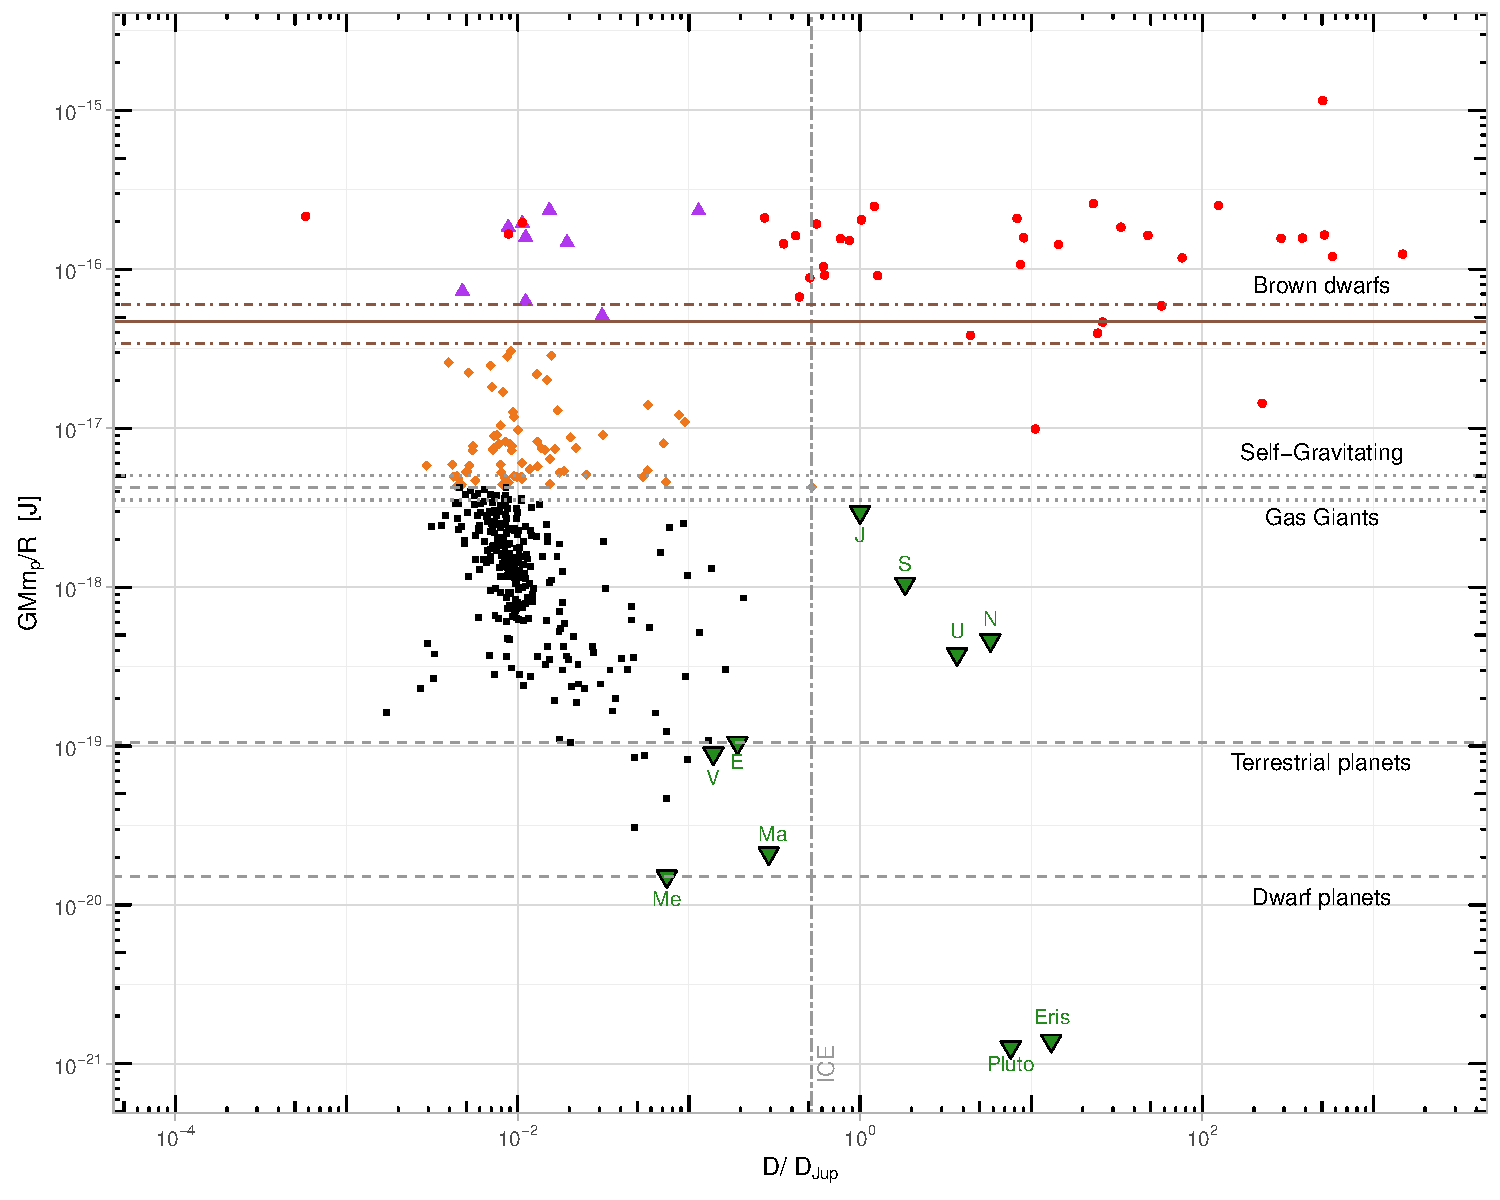
\includegraphics[width=0.85\linewidth]{f01.pdf}
\caption{The BGP diagram for exoplanets and BDs: nSGEs (black squares), SGEs (orange diamonds),  and BDs (red solid dots); the SGEs falling in BD region are identified by purple triangles. The inverted green triangles correspond to the positions occupied by the different kinds of planets in the solar system. The position of the ice line (or water "snowline") in the solar system (vertical dot-dash line) is also indicated. \citep{Torres2016}}
\label{fig:figTor1}
\end{figure}

In Figure~\ref{fig:figTor1} (hereafter, the BGP diagram) authors compare for the exoplanets (black squares and orange diamonds) and BDs (red solid dots) the BGP and distances from their companion stars, as normalized by the distance of Jupiter from the sun (${\rm D}/{\rm D_{Jup}}$). The BGP diagram is separated in four zones, synonymous with different physical structures. The upper zone is defined by the lower mass limit of $13\ M_{Jup}$ for the burning of deuterium in BDs. 

A few exoplanets are located above the deuterium-burning limit, while a few BDs are below this limit, suggesting that the deuterium-burning criterion does not allow a clear distinction between these two objects. Also, as observed by \citet{Santerne2016}, many BDs in this sample are found at a distance nearer than Jupiter from the Sun, that is in disagree with the BD's desert hypothesis. 
Therefore, although the majority of the exoplanets and BDs occupy different regions in the BGP diagram, their separation in terms of physical structures is still somewhat ambiguous.   

\begin{figure}[!ht]
\centering
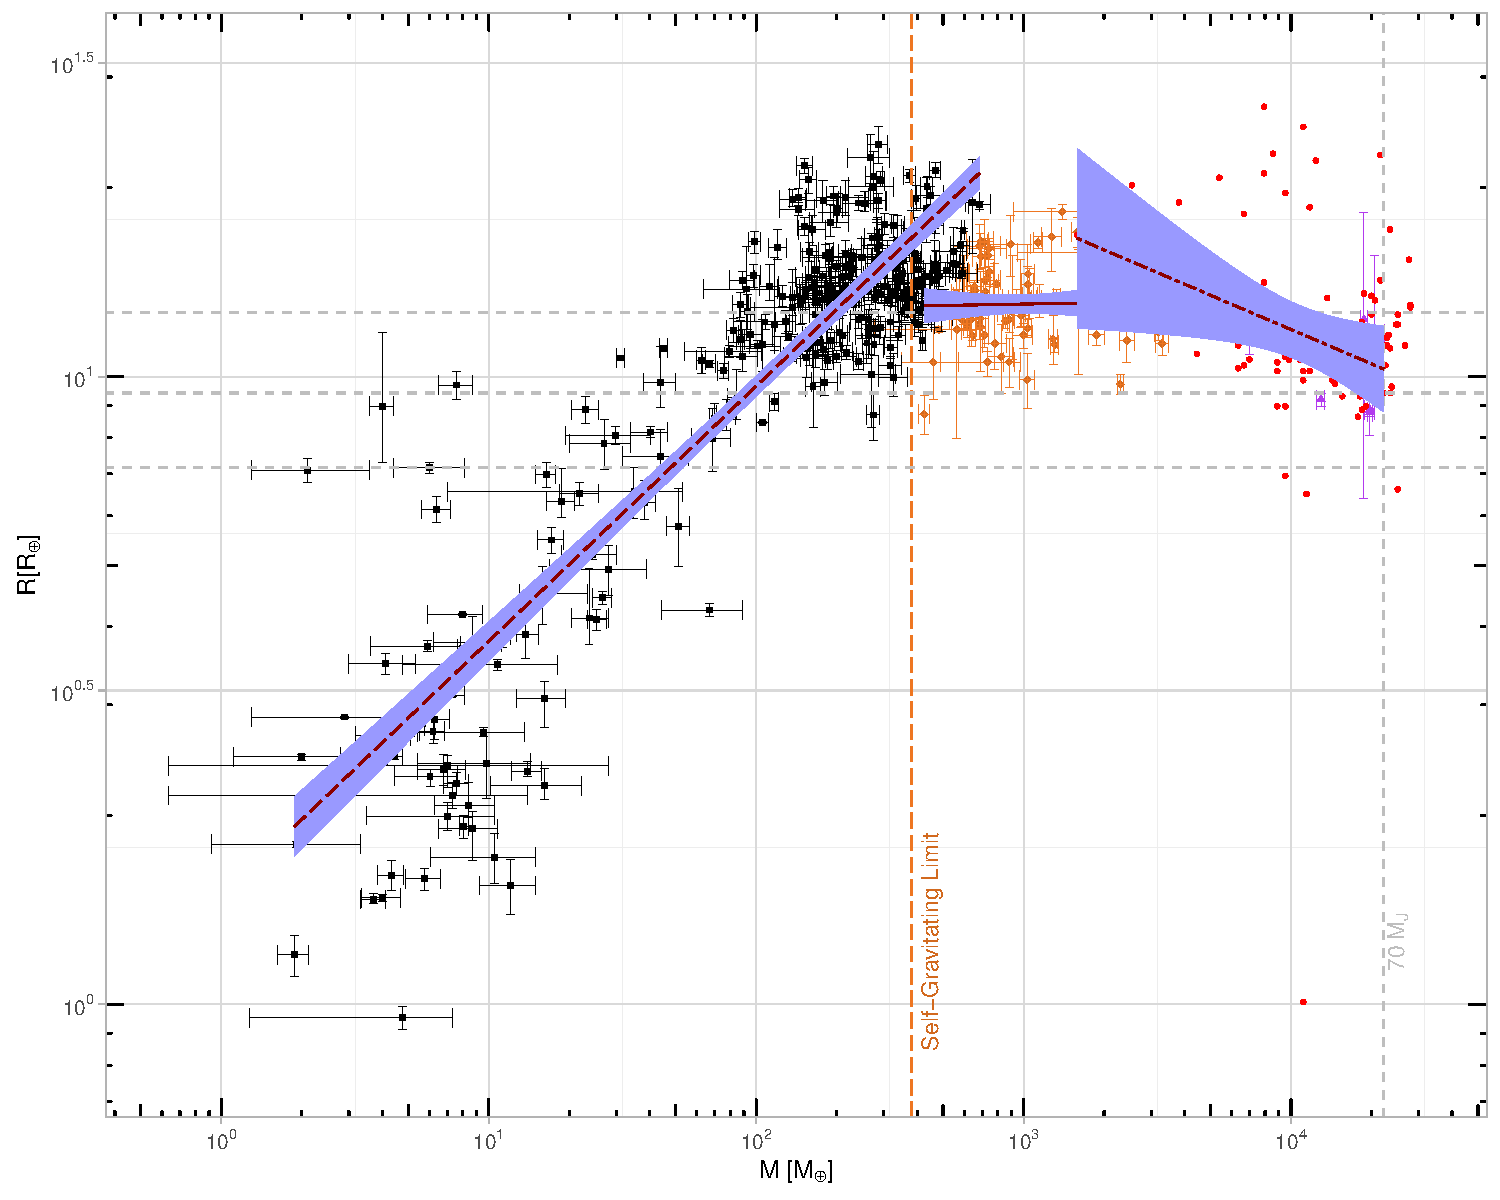
\includegraphics[width=0.85\linewidth]{f02.pdf}
\caption{Comparing the MRRs of exoplanets and BDs. The symbols are the same as in Fig. \ref{fig:figTor1}. Also shown are the critical mass at the SG limit and the upper mass limit $70~M_{Jup}$ for BDs.}\
\label{fig:figTor2}
\end{figure}

Based on the Self-Gravitating (SG) limit, separation on the gas-giant exoplanets in Self-Gravitating (SGE) and non Self-Gravitating (nSGE) was made.   
The BGP for the SG limit is defined by a critical mass, $M_c=1.2 M_{Jup}$, and critical radius, $R_c=0.84 R_{Jup}$ \citep{Padmanabhan1993}. 
Although both $M_c$ and $R_c$ are typical values 
for massive exoplanets, the critical mass is also comparable with the 
theoretical lowest mass expected for a BD, while the critical radius
is consistent with their observed mean radius \citep{Burgasser2008,Basri2006,Sorahana2013}.  

According to \citet{Padmanabhan1993}, the MRRs of 
bodies with different structures would be expected to change abruptly at the 
SG limit, from a positive MRR below the SG limit, to a negative one above it, which may help to separate exoplanets and BDs. 
This be observed on Figure~\ref{fig:figTor2}, where MRRs for the exoplanets and BDs are compared: the nSGEs show a positive MRR while the BDs show a negative one (see Table~\ref{tab:Tor1}). On the other hand, the SGEs show a relation where the radius does not increase with the mass. This characteristics was also observed by \citet{Hatzes2015}, although these authors did not offered any physical explanation for this behavior. 

\begin{table}[t]
\centering
\caption{Linear regression in log, $(R/R_{\oplus}) = 10^{b}\times (M/M_{\oplus})^a$, and their coefficients of correlation $r^2$.
Values from \cite{Torres2016}.}
\begin{tabular}{l c c c}
\noalign{\smallskip}\hline\hline\noalign{\smallskip}
\textbf{Sub-samples} & \textbf{a} & \textbf{b} & $r^2$\\
\noalign{\smallskip}\hline\noalign{\smallskip}
%SSP & $+0.29 \pm 0.01$ & $0.00 \pm 0.02$ & 0.995 \\
nSGE & $+0.41 \pm 0.01$ & $0.17 \pm 0.03$ & 0.785 \\
SGE & $+0.01 \pm 0.03$ & $1.09 \pm 0.10$ & 0.001 \\
BD & $-0.18 \pm 0.08$ & $1.60 \pm 0.33$ & 0.069 \\
\noalign{\smallskip}\hline
\end{tabular}
\label{tab:Tor1}
\end{table}

For the SGEs, we interpret the radius that shows no significant change as the mass increases as evidence for the presence of a dominant liquid metallic hydrogen (LMH) envelop \citep{Wigner1935,Hubbard1997,Dalladay-Simpson2016}: this is due to the very low compressibility of LMH \citep{Hubbard1997}. 

It was suspected by many authors that gas-giant planets, 
like Jupiter and Saturn in the solar system, have a LMH envelope \citep[see][and reference therein]{Burrows1993}. 
But, one would not expect to observe evidence for such envelopes. This is because, although the LMH layer could constitute 50\% to 85\% of the 
mass of a gas-giant planet, this layer would generally be hidden below a rich envelope of hydrogen gas. 
As the mass of a gas-giant exoplanet increased above the critical mass, $M_c$, the self-gravity of 
matter became more important, the pressure increased and most of 
the hydrogen in the outer gas envelope changed phase, transforming into LMH. 
Alternatively, since most of these exoplanets are Hot Jupiters with high eccentricities, they might have lost their outer envelop of gas when passing near their stars, revealing their underlying LMH envelopes \citep{Torres2016}. 

\begin{figure}[ht]
\centering
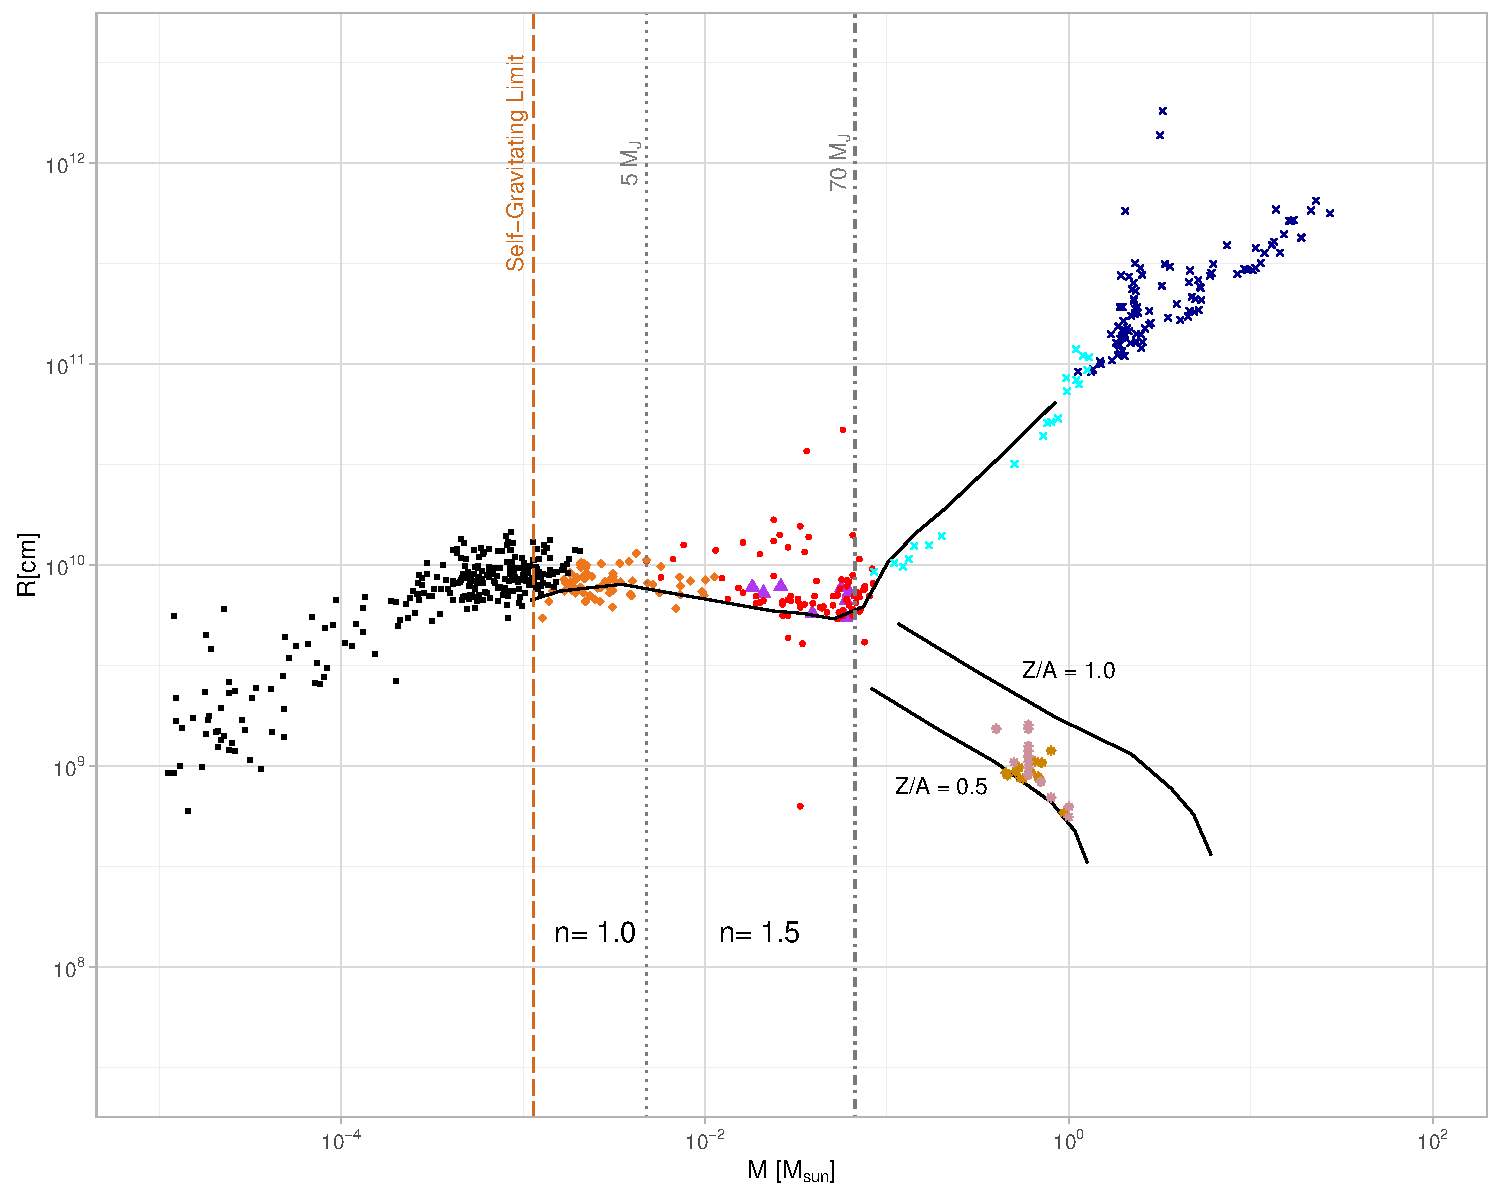
\includegraphics[width=0.85\linewidth]{f05.pdf}
\caption{Model of BDs formed of LMH. 
The MRR for the very low-mass stars (VLM, in light blue) becoming positive as they evolve towards the main sequence (dark blue x), 
while the MRR for WDs (white dwarfs, brown squares) is still negative. 
Two MRR for WDs, with different hydrogen richness (Z/A = 0.5 and Z/A = 1.0), are also represented. }
\label{fig:figTor3}
\end{figure}

However, based on the LMH interpretation there is still another alternative, which is that above the SG limit, objects are really BDs. In Figure~\ref{fig:figTor3} \citeauthor{Torres2016} compare their data with the predictions made by such a model, as developed by \citet{Burrows1993}. In this model BDs are formed at 99.9\% of 
LMH, this percentage decreasing as the mass of the star decreases, down to the SG limit. Below $5\ M_J$, the Coulomb correction competes 
with the degeneracy component, and the polytropic index, $n$, changes 
from 1.5 to 1.0, making the radius independent from the mass. 
According to this model, even above $5\ M_J$, 
when $n = 1.5$ and $R \propto M^{-1/3}$, the dependence of the radius on 
the mass would be weak, that corresponds to the low coefficients of correlation that was observed.  
According to this interpretation, therefore, it would be difficult, if not impossible, to distinguish between BDs and massive exoplanets. \citep{Torres2016}. 
While BD's appear to form preferentially like stars, from the graviturbulent fragmentation of a parent molecular clump, GP's form essentially by core accretion in a protoplanetary disk, i.e. from the grow of solids yielding eventually the accretion of a surrounding gas rich H/He envelope. So the definition of BD or GP is tightly linked with a processes of its formation mechanism.      
% % % % % % % % % % % % % % % % % %

\section{Detection of Exoplanets and Brown Dwarfs}
Several of the search methods for extrasolar planets and brown dwarfs are similar to those employed to
search for eclipsing and other periodic variable stars, but need to be more exact
because of the low amplitudes involved. At present, there is one direct and several indirect
methods available in the search for extrasolar planets which are discussed below.

\begin{itemize}
\item Direct (imaging/spectroscopy). In optical and infrared spectral regions, we can look for faint companions of
nearby stars, but true planets are not likely to be luminous enough to
be seen directly. It is even more difficult to obtain high spectral resolution 
to discern identifying features in the spectrum of any such candidate objects.
The difficulty is that the overwhelming light of the parent star makes it very difficult to
separate the flux of the planet from its star. Coronagraphic \citep{lyot1933}
and diffraction techniques are beginning to yield results as new generation space telescopes 
are an obvious answer to this need, but high resolution
techniques on existing telescopes may permit detection sooner \citep{milone2014}.

\item Astrometric variations.
Proper motions are secular angular motions in the plane of the sky, usually
expressed in units of arcsec/year in coordinates such as right ascension and declination.
They indicate slight changes in the direction of the star as seen from the Sun.
The size of this motion depends on the object's distance as well as the object's
linear motion across the line of sight. Periodic variation in the proper motion of
an object is a sign of binarity.
The method is applicable to any low-mass companions, and so to brown dwarfs
and planets as well as stars (astrometric binaries).

The amplitude of the variation depends on the ratio of the masses of the objects, which is inversely
proportional to the separation of the two objects from the centre of mass of the system.
If the mass of the system is known, for example, through a well-calibrated
mass-luminosity relation, the mass of the companion can be determined \citep{milone2014}.

\item Transits. While the radial velocity method provides information about a planet's mass, the photometric method can determine the planet's radius. This is the main advantage of the transit method. If a planet crosses (transits) in front of its host star's disk, then the observed visual brightness of the star drops by a small amount that depend on the relative sizes of the star and the planet. For example, in the case of HD 209458, the host star is dimmed by 1.7\%.

This method has two major disadvantages. First, planetary transits are only observable when the planet's orbit happens to be perfectly aligned from the astronomers vantage point. The probability of a planetary orbital plane being directly on the line-of-sight to a star is the ratio of the diameter of the star to the diameter of the orbit (in the case of small stars, the radius of the planet is also an important factor).
The second disadvantage of this method is a high rate of false detections. A 2012 study found that the rate of false positives for transits observed by the Kepler mission could be as high as 35\%-40\% in single-planet systems \citep{Santerne2012}. For this reason, a star with a single transit detection requires additional confirmation, typically from the radial-velocity method \cite{milone2014}.

\item Transit time variations.
Method for detecting exoplanets by observing variations in the timing of a transit. This provides an extremely sensitive method capable of detecting additional planets in the system with masses potentially as small as the Earth. In tightly packed planetary systems, the gravitational pull of the planets among themselves causes one planet to accelerate and another planet to decelerate along its orbit. The acceleration causes the orbital period of each planet to change. Detecting this effect by measuring the change is known as Transit Timing Variations.

\item Gravitational lensing. Unlike most other planet-detection techniques, gravitational microlensing
does not rely on detection of photons from either the host or the planet. Planets are discovered 
by their gravitational perturbation of light from a more distant source.

The most important attributes of the microlensing method are: (a) its sensitivity to planets orbiting
host stars with a broad range of masses located over a large range of Galactocentric distances;
(b) its sensitivity to low-mass planets, planets in wide orbits, free-floating planets, and, in particular,
planets with orbits at or beyond the so-called snow line (the location in the protoplanetary disk
where the disk midplane temperature is below the sublimation temperature of water); (c) the
fact that microlensing events and planetary perturbations are stochastic, rare, and unpredictable.

Microlensing detects planets through the instantaneous gravitational perturbation of the light
rays of a source star by the planet, as opposed to methods such as radial velocity or astrometry,
which require a full planet orbit to detect the gravitational influence of the planet on its host star.
Furthermore, when detected in conjunction with the microlensing event caused by its host star,
planets typically perturb light rays that pass close to the angular Einstein ring radius of the host
lens,
\begin{equation} \label{eq:ml_ring}
\theta_{E}\equiv \left( \dfrac{4GM}{D_{rel}c^{2}} \right) 
\end{equation}
where $M$ is the mass of the (host) lens, $D^{−1}_{rel} \equiv D^{−1}_{l} - D^{−1}_{s}$, and $D_{l},D_{s}$ 
are the distances to the lens and source \citep{gaudi2012}.

\item Radial velocity variations. 
A star with a planet will move in its own small orbit in response to the planet's gravity. This leads to variations in the speed with which the star moves toward or away from planet, i.e. the variations are in the radial velocity of the star with respect to planet. The radial velocity can be deduced from the displacement in the parent star's spectral lines due to the Doppler effect. The radial-velocity method measures these variations in order to confirm the presence of the planet using the binary mass function.

The speed of the star around the system's centre of mass is much smaller than that of the planet, because the radius of its orbit around the centre of mass is so small. However, velocity variations down to 1 m/s or even somewhat less can be detected with modern spectrometers, such as the HARPS spectrometer at the ESO 3.6 meter telescope in La Silla Observatory, Chile, or the HIRES spectrometer at the Keck telescopes.

Until 2014, the radial-velocity method was by far the most productive technique used by planet hunters. It is also known as Doppler spectroscopy. The method is distance independent, but requires high signal-to-noise ratios to achieve high precision, to find lower-mass planets. This method easily finds massive planets that are close to stars. Modern spectrographs can also easily detect Jupiter-mass planets orbiting 10 astronomical units away from the parent star, but detection of those planets requires many years of observation.

Planets with orbits highly inclined to the line of sight from Earth produce smaller visible wobbles, and are thus more difficult to detect. 
One of the advantages of the radial velocity method is that eccentricity of the planet's orbit can be measured directly. One of the main disadvantages of the radial-velocity method is that it can only estimate a planet's minimum mass.

\item Indirect effects on (O-C) diagrams of EBs.
Times of minimum light from EB constitute a time stamp on the system. If there is a planet in circumbinary orbit around the binary stars, the stars
will be offset around a binary-planet centre of mass. As the stars in the binary are displaced back and forth by the planet, the times of the
eclipse minima will vary. 
The periodicity of this offset may be the most reliable way to detect extrasolar planets around 
close binary systems \citep{deeg2000, doyle1998}. With this method, planets are more easily detectable 
if they are more massive, orbit relatively closely around the system, and if the stars have low masses.

The eclipsing timing method allows the detection of planets further away from the host star than the transit method. 
%However, signals around cataclysmic variable stars hinting for planets tend to match with unstable orbits \citep{horner2013}. 
In 2011, Kepler-16b became the first planet
to be definitely characterized via eclipsing binary timing variations \citep{doyle2011}.

Proto-planetary disks have been seen around several stars, including $\beta$ Pictoris
and Vega, and remnants of disks have been seen around older stars. Gaps and
warping have been attributed to the presence of planets or proto-planets in some of
these systems \cite{milone2014}.
\end{itemize}


